
\documentclass[a4paper,12pt, oneside]{book}

%  Русский язык
\usepackage{cmap}					% Улучшенный поиск русских слов
\usepackage[T2A]{fontenc}			% кодировка
\usepackage[utf8]{inputenc}			% кодировка исходного текста
\usepackage[english,russian]{babel}	% локализация и переносы
\usepackage{pscyr}					% нормальные шрифты

% Колонтитулы
\usepackage{fancybox,fancyhdr}
\usepackage{lastpage}
\fancyhf{}
\fancypagestyle{all}
{
	\fancyhead{}
	\fancyhead[C]{\vspace{-5mm}Контрольная работа 12 Вариант Попов Юрий СКБ-171\vspace{3mm}}
	\fancyfoot{}
	\fancyfoot[C]{\hfill  \thepage  \hfill}
}

% Картинки и графики
\usepackage{wrapfig}
\usepackage{pgfplots}
\pgfplotsset{compat=1.9}

% Ссылки
\usepackage{xcolor}
\usepackage{color,colortbl} % раскраска таблиц
\usepackage[unicode, pdftex]{hyperref}
\definecolor{linkcolor}{HTML}{000000} 	% цвет ссылок
\definecolor{urlcolor}{HTML}{8B000F}	% цвет гиперссылок
\hypersetup{urlcolor=urlcolor, linkcolor=linkcolor, colorlinks=true}

% Размеры
\setlength{\paperwidth}{210mm}
\setlength{\paperheight}{297mm}
\setlength{\textheight}{225mm} 			% высота без колонтитулов
\setlength{\textwidth}{170mm}			% ширина текста
\oddsidemargin=0pt
\setlength{\headheight}{2mm}			% высота колонтитула
\setlength{\headsep}{5mm} 	% от блока текста до верхнего колонтитула
\setlength{\footskip}{10mm}  % от блока текста до нижнего колонтитула

% Математика
\usepackage{mathrsfs} % Красивый матшрифт
\usepackage{amsmath,amsfonts,amssymb,amsthm,mathtools,mathtext} 
\usepackage{latexsym,array,epsfig,wasysym}
\usepackage[all]{xy}
\let\int\varint
\def\Int{\int\limits}
\def\IInt{\iint\limits}
\def\IIInt{\iiint\limits}
\DeclarePairedDelimiter\floor{\lfloor}{\rfloor}


% Оглавление 
\usepackage{setspace}

\usepackage{tocloft} %регулировка расположения TableOfContent (Оглавления) на странице

%\setcounter{tocdepth}{1} % отменяет вывод в оглавление subsection and subsubsection
%\setcounter{secnumdepth}{1} %отменяет номерацию секций в тексте и оглавлении.
\usepackage{tocloft} %регулировка расположения TableOfContent (Оглавления) на странице

\renewcommand{\cfttoctitlefont}{\hspace{0.38\textwidth} \bfseries\MakeUppercase} %уменьшаем размер шрифта и ровняем по центру

% % Межстрочные отступы в Оглавлении:
\setlength{\cftbeforetoctitleskip}{5mm} %отступ Оглавления от верхнего поля страницы.
\setlength{\cftbeforechapskip}{14mm} %отступ между главами
\setlength{\cftbeforesecskip}{5mm} %отступ между секциями \section{title}

% % Отступы от левого поля:
\setlength{\cftchapindent}{1mm} %отступ между левым полем и \chapter{}
\setlength{\cftsecindent}{13mm} %отступ между левым полем и \section{title}

% % Отточия в Оглавлении
\renewcommand\cftchapdotsep{\cftdot} %добавляет отточия после \chapter{title}
%\renewcommand{\cftchapleader}{\cftdotfill{\cftchapdotsep}} %делает отточия после \chapter{title} тонкими, (по умолчанию жирные).
\renewcommand\cftsecdotsep{\cftdot} %делает отточия после \section{title} частыми.

% % Интервалы между абзацами, главами и так далее:
\usepackage{titlesec}

\titleformat{\chapter}[display]
{\filcenter}
{\MakeUppercase{\chaptertitlename} \thechapter}
{8pt}
{\bfseries}{}

\titleformat{\section}
{\normalsize\bfseries}
{\thesection}
{1em}{}

\titleformat{\subsection}
{\normalsize\bfseries}
{\thesubsection}
{1em}{}

% Настройка вертикальных и горизонтальных отступов
\titlespacing*{\chapter}{0pt}{-30pt}{8pt}
\titlespacing*{\section}{\parindent}{*4}{*4}
\titlespacing*{\subsection}{\parindent}{*4}{*4}


\begin{document} % начало документа	
	\pagestyle{plain}
	
	\begin{titlepage}	
		\begin{center}
			{\Huge \textbf{Математическая статистика}}
			\vspace{30mm}
			
			{\Huge Домашняя работа № 4 \\}
			\vspace{30mm}
			
			{\huge Проверка статистических гипотез}
			\vspace{30mm}
			
			{\Large Попов Юрий, СКБ-172}
		\end{center}
	\end{titlepage}
	
	
	
	\begin{spacing}{0.99}          
		\tableofcontents %Оглавление. Корректно создается за два прогона tex файла.               
	\end{spacing}

\newpage
\begin{center}
	{\Huge{\bf{Предисловие}}}
\end{center}


%-------------------------------------Предислов

\setcounter{secnumdepth}{-1} % убираем нумерацию 


%-------------------------------------Предисловие
\newpage

\begin{center}
	\textbf{\Large Немного теории}
\end{center}

\normalsize{\textbf{Определение 1}} \textit{ Статистическая гипотеза } - это некоторое предположение о виде или параметрах распределений\\

\normalsize{\textbf{Определение 2}} \textit{ Статистический критерий  } - это правило, по которому каждой реализации выборки ставится в соответствие решение: принимаем гипотезу $ H_0 $ или отвергаем ее( то есть принимаем гипотезу $ H_1 $)\\

\normalsize{\textbf{Определение 3}} \textit{ Уровень значимости статистического теста } - допустимая для данной задачи вероятность ошибки первого рода, то есть вероятность отклонить нулевую гипотезу, когда на самом деле она верна\\

\normalsize{\textbf{Определение 4}} В случае, когда $ H_0 $ и $ H_1 $ - простые гипотезы, $ P(x \in \mathcal{F} | H_0)) = \lambda $ - {\it ошибка 1 рода}

$ \beta = P(H_0 | H_1) $ - \textit{ошибка второго рода}\\

\normalsize{\textbf{Определение 5}} Если $ H_0 $ состоит из одного определения, то говорят, что $ H_0 $ - \textit{простая гипотеза}, иначе $ H_0 $  \textit{сложная гипотеза}\\

\normalsize{\textbf{Определение 6}} Если $ H_1 $ состоит из одного определения, то говорят, что $ H_1 $ - \textit{простая гипотеза}, иначе $ H_1 $  \textit{сложная гипотеза}\\

\normalsize{\textbf{Определение 7}} \textit{ Функция мощности критерия } - это функционал на множестве допустимых распределений  $ \mathcal{F} $  и выборке $ X $

\newpage
\begin{center}
	\textbf{\Large Перейдем к практике}
\end{center}

\chapter{4.1 Проверка гипотезо виде распределений}


\section{Критерий согласия хи квадрат}
\begin{center}
	{\large Свойства данного критерия:}
\end{center}


\textbf{Положительные стороны:}\\

Возможность применения как для дискретных, так и для непрерывных случайных величин, а так же отсутствие необходимости учитывать точные значения наблюдений (бывают случаи, когда исходные данные имеют не
числовой характер), простота и наглядность.\\

\textbf{Недостатки:}\\

Недостатком этого критерия является тот факт, что в случае применения его для непрерывных распределений используется группировка наблюдений, приводящая к рассмотрению дискретной схемы, что приводит к некоторой потере информации, а также к необходимости рассмотрения вопроса о виде и числе интервалов.


\section{Критерий согласия Колмогорова - Смирнова}

\begin{center}
	{\Large Свойства данного критерия:}
\end{center}


\textbf{Положительные стороны:}\\

Сильной стороной этого критерия является то, что, имея таблицы значений функции
Колмогорова $ K(t) $, мы можем рассчитывать критерий для проверки гипотезы относительно
произвольной непрерывной функции распределения $F(x)$\\

\textbf{Недостатки:}\\

Недостатком является то, что он работает только для непрерывных распределений, по своей сути он является асимптотическим и , при его применении учитывается лишь наибольшее расхождение между эмпирической и теоретической функциями распределения, т.е. используется не вся информация. Оценка согласия по одной точке, особенно при небольшой длине выборки может плохо отражать соответствие эмпирических данных теоретическому закону распределения

\section{4.1.1 Геометрическое распределение}

\subsection{Критерий согласия хи-квадрат для простой гипотезы}

Проверим с помощью $ \chi^2 $  - критерия Пирсона нулевую гипотезу$ H_0 $ = (Наша выборка распределена по геометрическому закону), то есть $ p_k = P(X = k ) = p (1-p)^k, k = 0,1, \ldots $, при соответствующем уровне значимости\\ 

Для начала вычисляем выборочное среднее. Так как в этом случае у нас простоя гипотеза, то мы просто подставляем значение параметра. Я взял $ p = 0.2 $\\

Затем, я посчитал теоретические вероятности и теоретические частоты по соответствующим  формулам:\\
$$ 
p_k = 0.2 (1 - 0.2)^k 
$$
и
$$
n_k' = n p_k
$$  


Затем я рассчитал меру отклонения Пирсона для каждого значения и составил итоговую таблицу:

\begin{figure}[h!]
	\begin{center}
		\begin{minipage}[h]{0.47\linewidth}
			\center{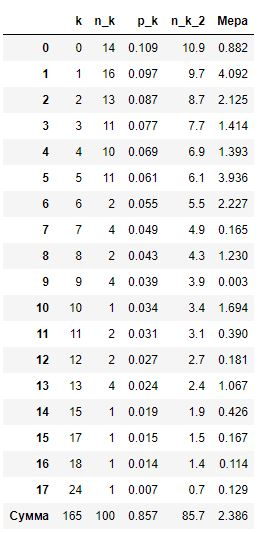
\includegraphics[width=1\linewidth]{fotos/geom/Pirson_prost}} n = 100 \\
		\end{minipage}
	\end{center}
\end{figure}


\newpage
Из расчетной таблицы видно значение критерия Пирсона $ \chi^2 \text{(правый нижний угол)} = 0.127$. 

\subsubsection{Уровень значимости равен 0.1}

Критическая точка для уровня значимости 0.1 при количестве степеней свободы $ k = 15(16 - 1) $ равна $22,30712$\\

Так как наблюдаемое значение критерия меньше меньше критического, то нет основания отвергнуть нулевую гипотезу о распределении нашей выборки по геометрическому закону с параметром $ p = 0.2 $.  



\subsubsection{Уровень значимости равен 0.05} 

Критическая точка для уровня значимости 0.05 при количестве степеней свободы $ k = 15(16 - 1) $ равна $24,99579014$\\

Так как наблюдаемое значение критерия меньше меньше критического, то нет основания отвергнуть нулевую гипотезу о распределении нашей выборки по геометрическому закону c параметром $ p = 0.2 $.  


\newpage
\subsection{Критерий согласия хи-квадрат для сложной гипотезы}

Проверим с помощью $ \chi^2 $  - критерия Пирсона нулевую гипотезу$ H_0 $ = (Наша выборка распределена по геометрическому закону), то есть $ p_k = P(X = k ) = p (1-p)^k, k = 0,1, \ldots $, при соответствующем уровне значимости\\ 


Для начала вычисляем выборочное среднее. В этом случае у нас сложная гипотеза, поэтому найдем оценку нашего параметра. В моем случае это $ p = \dfrac{1}{\overline{x}} $ . Оно получилась равна $ 0.104 $\\

Затем, я посчитал теоретические вероятности и теоретические частоты по соответствующим  формулам:\\
$$ 
p_k = 0.104 (1 - 0.104)^k 
$$
и
$$
n_k' = n p_k
$$  


Затем я рассчитал меру отклонения Пирсона для каждого значения и составил итоговую таблицу:

\begin{figure}[h!]
	\begin{center}
		\begin{minipage}[h]{0.47\linewidth}
			\center{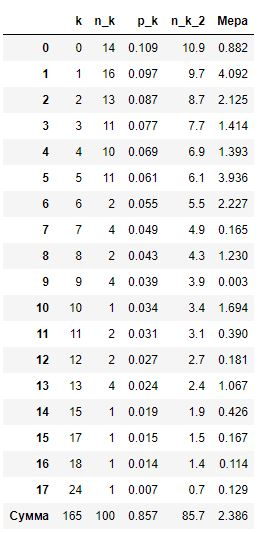
\includegraphics[width=1\linewidth]{fotos/geom/Pirson_slog}} n = 100 \\
		\end{minipage}
	\end{center}
\end{figure}


\newpage
Из расчетной таблицы видно значение критерия Пирсона $ \chi^2 \text{(правый нижний угол)} = 2.386$. 

\subsubsection{Уровень значимости равен 0.1}

Критическая точка для уровня значимости 0.1 при количестве степеней свободы $ k = 16(18 - 1 - 1) $ равна $23,54182892$\\

Так как наблюдаемое значение критерия меньше меньше критического, то нет основания отвергнуть нулевую гипотезу о распределении нашей выборки по геометрическому закону с оценкой параметра, равной $ p = 0.104 $   



\subsubsection{Уровень значимости равен 0.05} 

Критическая точка для уровня значимости 0.05 при количестве степеней свободы $ k = 16(18 - 1 - 1) $ равна $26,2962276$\\

Так как наблюдаемое значение критерия меньше меньше критического, то нет основания отвергнуть нулевую гипотезу о распределении нашей выборки по геометрическому закону с оценкой параметра, равной $ p = 0.104 $ .  





\newpage
\section{4.1.2 Экспоненциальное распределение}


\subsection{Критерий согласия хи-квадрат для простой гипотезы}

Проверим с помощью $ \chi^2 $  - критерия Пирсона нулевую гипотезу$ H_0 $ = (Наша выборка распределена по экспоненциальному закону), то есть $ p_k = P(X = k ) = \lambda e^{-\lambda k}, k = 0,1, \ldots $, при соответствующем уровне значимости\\ 

Мне было необходимо разбить мой интервал на промежутки, и посчитать сколько значений моей выборки попадает в каждый из промежутков. Я решил разбивать на интервалы так, чтобы в каждый из них попадало одинаковое количество чисел из моей выборки.\\

Соответственно, я разбил на интервалы и посчитал количество вхождений.\\

Затем вычислил выборочное среднее и, так как в этом случае у нас простая гипотеза, то взял значение параметра $ \lambda = 0.8 $

Затем, я посчитал теоритические вероятности попадания в интервалы и теоретические частоты по соответствующим  формулам:\\
$$ 
P_i = P(x_i < X < x_{i+1}) = e^{-\lambda x_i} - e^{-\lambda x_{i+1}} = e^{-0.8 x_i} - e^{-0.8 x_{i+1}}
$$
и
$$
n_k' = n p_k 
$$  


Затем я рассчитал меру отклонения Пирсона для каждого значения и составил итоговую таблицу:

\begin{figure}[h!]
	\begin{center}
		\begin{minipage}[h]{0.47\linewidth}
			\center{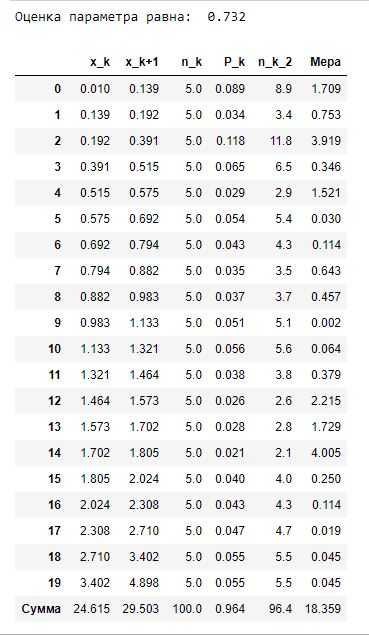
\includegraphics[width=1\linewidth]{fotos/expon/Pirson_prost}} n = 100 \\
		\end{minipage}
	\end{center}
\end{figure}


\newpage
Из расчетной таблицы видно значение критерия Пирсона $ \chi^2 \text{(правый нижний угол)} = 23.242$. 

\subsubsection{Уровень значимости равен 0.1}

Критическая точка для уровня значимости 0.1 при количестве степеней свободы $ k = 19 (20 - 1)$ равна $27,20357103$\\

Так как наблюдаемое значение критерия меньше меньше критического, то нет основания отвергнуть нулевую гипотезу о распределении нашей выборки по экспоненциальному закону  с параметром $ \lambda = 0.8 $.  



\subsubsection{Уровень значимости равен 0.05} 

Критическая точка для уровня значимости 0.05 при количестве степеней свободы $ k = 19 ( 20 - 1) $ равна $30,14352721$\\

Так как наблюдаемое значение критерия меньше меньше критического, то нет основания отвергнуть нулевую гипотезу о распределении нашей выборки по экспоненциальному закону с параметром $ \lambda = 0.8 $.  

\subsection{Критерий согласия хи-квадрат для сложной гипотезы}


Проверим с помощью $ \chi^2 $  - критерия Пирсона нулевую гипотезу$ H_0 $ = (Наша выборка распределена по экспоненциальному закону), то есть $ p_k = P(X = k ) = \lambda e^{-\lambda k}, k = 0,1, \ldots $, при соответствующем уровне значимости\\ 

Мне было необходимо разбить мой интервал на промежутки, и посчитать сколько значений моей выборки попадает в каждый из промежутков. Я решил разбивать на интервалы так, чтобы в каждый из них попадало одинаковое количество чисел из моей выборки.\\

Соответственно, я разбил на интервалы и посчитал количество вхождений.\\

Затем вычислил выборочное среднее и нашел оценку нашего параметра. В моем случае это $ \lambda = \dfrac{1}{\overline{x}} $ . Оно получилась равна $ 0.732 $\\

Затем, я посчитал теоритические вероятности попадания в интервалы и теоретические частоты по соответствующим  формулам:\\
$$ 
P_i = P(x_i < X < x_{i+1}) = e^{-\lambda x_i} - e^{-\lambda x_{i+1}} = e^{-0.732 x_i} - e^{-0.732 x_{i+1}}
$$
и
$$
n_k' = n p_k 
$$  


Затем я рассчитал меру отклонения Пирсона для каждого значения и составил итоговую таблицу:

\begin{figure}[h!]
	\begin{center}
		\begin{minipage}[h]{0.47\linewidth}
			\center{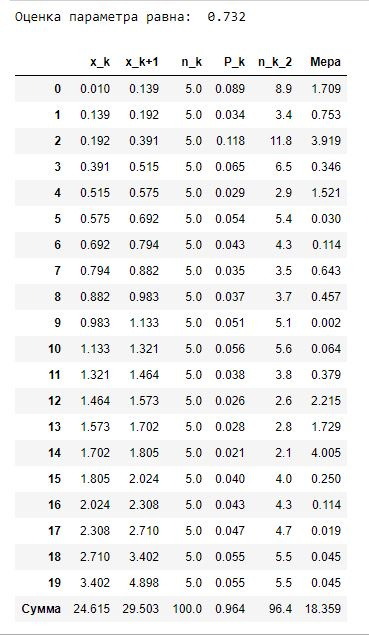
\includegraphics[width=1\linewidth]{fotos/expon/Pirson_sloq}} n = 100 \\
		\end{minipage}
	\end{center}
\end{figure}


\newpage
Из расчетной таблицы видно значение критерия Пирсона $ \chi^2 \text{(правый нижний угол)} = 18.359$. 

\subsubsection{Уровень значимости равен 0.1}

Критическая точка для уровня значимости 0.1 при количестве степеней свободы $ k = 18(20 - 1 - 1) $ равна $25,98942308$\\

Так как наблюдаемое значение критерия меньше меньше критического, то нет основания отвергнуть нулевую гипотезу о распределении нашей выборки по экспоненциальному закону c оценкой параметра, равной $ \lambda = 0.732 $ .  



\subsubsection{Уровень значимости равен 0.05} 

Критическая точка для уровня значимости 0.05 при количестве степеней свободы $ k = 18 (20 - 1 - 1) $ равна $28,86929943$\\

Так как наблюдаемое значение критерия меньше меньше критического, то нет основания отвергнуть нулевую гипотезу о распределении нашей выборки по экспоненциальному закону c оценкой параметра, равной $ \lambda = 0.732 $ .  







\subsection{Критерий согласия Колмогорова - Смирнова для простой гипотезы}

Пусть дана выборка $X = (X_1 \ldots X_n)$ из распределения $\mathscr{L}(\xi)$ и $F_\xi$ - неизвестное распределение.

\begin{itemize}
	\item $H_0 : F_\xi = F(x)$ - простая гипотеза
	\item $H_1$ : не $F(x)$
\end{itemize}
Критерий Колмогорова основан на теореме Колмогорова:
\[
D_n = D_n(x) = \underset{x \in \mathop{R}}{\sup } |\hat{F}_n(x) - F(x) |
\]
где $D_n$ - это отклонение эмпирической функции распределения от теоретической функции распределения.
\\
$\hat{F}_n$ - оптимальная несмещенная состоятельная оценка для $F(x)$
\\

\subsection{Критерий согласия Колмогорова - Смирнова для сложной гипотезы}







\chapter{4.2 Задание для рассматриваемых распределений}

\section{4.2.1 Геометрическое распределение}

\section{4.2.2 Экспоненциальное распределение}







\begin{thebibliography}{99}
	\bibitem{rt1} 
	\bibitem{rt2} \href{http://www.complexdoc.ru/ntdpdf/541018/prikladnaya_statistika_pravila_proverki_soglasiya_opytnogo_raspredeleniya.pdf}{ссылка1}
	\bibitem{rt3}  \href{https://www.statisticshowto.datasciencecentral.com/exponential-distribution/}{ссылка2}
	\bibitem{rt4}  // \href{http://www.ams.jhu.edu/~dan/550.435/notes/COURSENOTES435.pdf}{ссылка3}
	\bibitem{rt5}  // \href{http://www.obzh.ru/nad/4-3.html}{ссылка4}
\end{thebibliography}

\end{document}
